% Written by projects/maia-calibration/paper/generate.mjs; do not edit by hand.

\newcommand{\AppCommit}{\texttt{ad7fa98}}
\newcommand{\Draws}{1{,}000}
\newcommand{\Seed}{7}
\newcommand{\MinFitMoves}{300}
\newcommand{\LichessMoves}{25{,}000}
\newcommand{\LichessGames}{13{,}785}
\newcommand{\FitMoves}{12{,}474}
\newcommand{\HeldMoves}{12{,}526}
\newcommand{\HisMoves}{33{,}522}
\newcommand{\HisGames}{640}
\newcommand{\KeptOffset}{250}
\newcommand{\PunishExact}{521}
\newcommand{\PunishAll}{684}
\newcommand{\PunishGames}{60}
\newcommand{\BenchMonth}{June 2025}
\newcommand{\BenchPerBand}{5{,}000}
\newcommand{\BenchPerGame}{8}
\newcommand{\BenchSeen}{150{,}181}
\newcommand{\BenchMinPly}{11}
\newcommand{\BenchMinClock}{30}
\newcommand{\BenchGapMin}{3.0}
\newcommand{\BenchGapMax}{3.9}
\newcommand{\BenchTop}{51.5}
\newcommand{\BenchConf}{54.9}
\newcommand{\FirstChoice}{12{,}875}
\newcommand{\TestTable}{%
\begin{tabular}{lrrrl}
\toprule
test & raw & tempered & tempered $-$ raw & \\
\midrule
1. Lichess, held-out half (log-likelihood per move) & $-$1.4944 & $-$1.4915 & 0.0029 [0.0014, 0.0044] & passes \\
2. the player's games (log-likelihood per move) & $-$1.3959 & $-$1.4026 & $-$0.0068 [$-$0.0079, $-$0.0057] & fails \\
3. punish events, verified (Brier score) & 0.1527 & 0.1542 & 0.0015 [$-$0.0005, 0.0037] & passes \\
\phantom{3.} punish events, all (Brier score) & 0.1550 & 0.1563 & 0.0013 [$-$0.0005, 0.0032] & \\
\bottomrule
\end{tabular}
}
\newcommand{\TestOneDiff}{0.0029}
\newcommand{\TestOneCI}{[0.0014, 0.0044]}
\newcommand{\TestTwoLoss}{0.0068}
\newcommand{\TestTwoLossCI}{[0.0057, 0.0079]}
\newcommand{\TestThreeDiff}{0.0015}
\newcommand{\TestThreeCI}{[$-$0.0005, 0.0037]}
\newcommand{\TestThreeAllDiff}{0.0013}
\newcommand{\TestThreeAllCI}{[$-$0.0005, 0.0032]}
\newcommand{\PunishRaw}{0.153}
\newcommand{\PunishTempered}{0.154}
\newcommand{\TempMin}{1.02}
\newcommand{\TempMax}{1.13}
\newcommand{\FitMovesMin}{620}
\newcommand{\TempFigure}{%
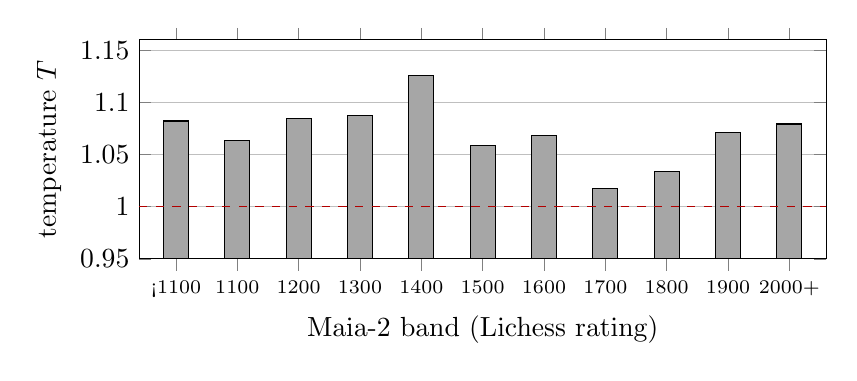
\begin{tikzpicture}
\begin{axis}[ybar, bar width=9pt, width=0.85\textwidth, height=0.36\textwidth, ymin=0.95, ymax=1.16,
  xmin=-0.6, xmax=10.6, xtick={0,1,2,3,4,5,6,7,8,9,10}, xticklabels={{<1100},{1100},{1200},{1300},{1400},{1500},{1600},{1700},{1800},{1900},{2000+}}, xticklabel style={font=\scriptsize},
  ylabel={temperature $T$}, xlabel={Maia-2 band (Lichess rating)}, ymajorgrids, enlarge x limits=false,
  y tick label style={/pgf/number format/fixed, /pgf/number format/precision=2}]
\addplot[fill=black!35, draw=black] coordinates {(0,1.0822) (1,1.0639) (2,1.0847) (3,1.0878) (4,1.1254) (5,1.0583) (6,1.0682) (7,1.0179) (8,1.0339) (9,1.0709) (10,1.0793)};
\draw[dashed, red!70!black] (axis cs:-0.6,1) -- (axis cs:10.6,1);
\end{axis}
\end{tikzpicture}
}
\newcommand{\LichGapMin}{2.0}
\newcommand{\LichGapMax}{5.2}
\newcommand{\LichTGapMin}{$-$1.1}
\newcommand{\LichTGapMax}{3.4}
\newcommand{\HisGapMin}{$-$1.3}
\newcommand{\HisGapMax}{1.1}
\newcommand{\HisTGapMin}{1.8}
\newcommand{\HisTGapMax}{4.6}
\newcommand{\HisBandLow}{<1100}
\newcommand{\HisBandHigh}{1400}
\newcommand{\GapFigure}{%
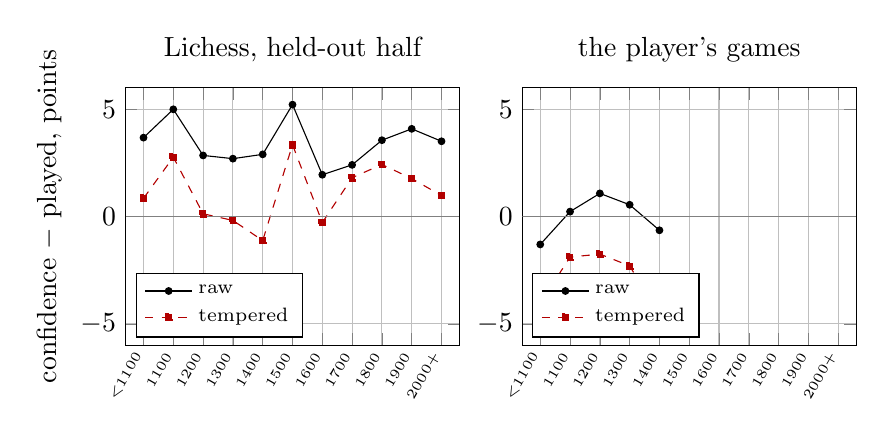
\begin{tikzpicture}
\begin{axis}[name=lichess, ylabel={confidence $-$ played, points}, width=0.48\textwidth, height=0.4\textwidth, xmin=-0.6, xmax=10.6, ymin=-6, ymax=6,
  xtick={0,1,2,3,4,5,6,7,8,9,10}, xticklabels={{<1100},{1100},{1200},{1300},{1400},{1500},{1600},{1700},{1800},{1900},{2000+}}, xticklabel style={font=\tiny, rotate=60, anchor=east}, grid=major,
  title={Lichess, held-out half}, legend pos=south west, legend cell align=left, legend style={font=\scriptsize}]
\addplot[black, mark=*, mark size=1.2pt] coordinates {(0,3.68) (1,5.00) (2,2.85) (3,2.70) (4,2.90) (5,5.22) (6,1.95) (7,2.41) (8,3.56) (9,4.09) (10,3.51)};
\addlegendentry{raw}
\addplot[red!70!black, dashed, mark=square*, mark size=1.2pt] coordinates {(0,0.85) (1,2.77) (2,0.13) (3,-0.18) (4,-1.12) (5,3.35) (6,-0.28) (7,1.81) (8,2.43) (9,1.77) (10,0.98)};
\addlegendentry{tempered}
\draw[gray] (axis cs:-0.6,0) -- (axis cs:10.6,0);
\end{axis}
\begin{axis}[at={(lichess.east)}, anchor=west, xshift=0.8cm, width=0.48\textwidth, height=0.4\textwidth, xmin=-0.6, xmax=10.6, ymin=-6, ymax=6,
  xtick={0,1,2,3,4,5,6,7,8,9,10}, xticklabels={{<1100},{1100},{1200},{1300},{1400},{1500},{1600},{1700},{1800},{1900},{2000+}}, xticklabel style={font=\tiny, rotate=60, anchor=east}, grid=major,
  title={the player's games}, legend pos=south west, legend cell align=left, legend style={font=\scriptsize}]
\addplot[black, mark=*, mark size=1.2pt] coordinates {(0,-1.30) (1,0.23) (2,1.08) (3,0.55) (4,-0.64)};
\addlegendentry{raw}
\addplot[red!70!black, dashed, mark=square*, mark size=1.2pt] coordinates {(0,-4.04) (1,-1.89) (2,-1.75) (3,-2.30) (4,-4.62)};
\addlegendentry{tempered}
\draw[gray] (axis cs:-0.6,0) -- (axis cs:10.6,0);
\end{axis}
\end{tikzpicture}
}
\newcommand{\BandTable}{%
\begin{tabular}{lrrrrrrrrr}
\toprule
 & & & \multicolumn{3}{c}{Lichess, held-out half} & \multicolumn{4}{c}{the player's games} \\
\cmidrule(lr){4-6}\cmidrule(lr){7-10}
band & fitting moves & $T$ & played & raw & tempered & moves & played & raw & tempered \\
\midrule
<1100 & 2{,}537 & 1.082 & 46.2 & 49.8 & 47.0 & 6{,}618 & 53.0 & 51.7 & 48.9 \\
1100 & 729 & 1.064 & 49.2 & 54.2 & 52.0 & 5{,}906 & 54.1 & 54.3 & 52.2 \\
1200 & 833 & 1.085 & 51.3 & 54.2 & 51.5 & 6{,}893 & 53.1 & 54.1 & 51.3 \\
1300 & 946 & 1.088 & 52.2 & 54.9 & 52.0 & 13{,}222 & 54.6 & 55.2 & 52.3 \\
1400 & 814 & 1.125 & 53.1 & 56.0 & 52.0 & 883 & 56.5 & 55.9 & 51.9 \\
1500 & 823 & 1.058 & 49.2 & 54.4 & 52.5 &  & & & \\
1600 & 841 & 1.068 & 52.8 & 54.7 & 52.5 &  & & & \\
1700 & 1{,}001 & 1.018 & 55.2 & 57.6 & 57.0 &  & & & \\
1800 & 833 & 1.034 & 53.4 & 56.9 & 55.8 &  & & & \\
1900 & 620 & 1.071 & 53.3 & 57.4 & 55.1 &  & & & \\
2000+ & 2{,}497 & 1.079 & 54.2 & 57.7 & 55.2 &  & & & \\
\bottomrule
\end{tabular}
}
